\newpage
\subsubsection{Senkrechte Polarisation mit $\mu_r$}
\begin{center}
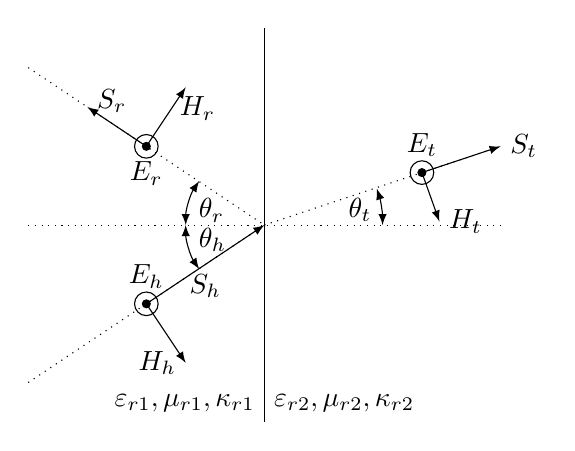
\begin{tikzpicture}
	\tikzset{cross/.style={cross out, draw=black, minimum size=2*(#1-\pgflinewidth), inner sep=0pt, outer sep=0pt},
		%     %default radius will be 1pt. 
		cross/.default={3.5pt}}
	%Kreuz
	\draw[dotted] (-3,0) -- (3,0);
	\draw[-] (0,2.5) -- (0,-2.5)                
	node[above right]   {$\varepsilon_{r2}, \mu_{r2}, \kappa_{r2}$}
	node[above left]    {$\varepsilon_{r1}, \mu_{r1}, \kappa_{r1}$};
	%Rücklaufende
	\draw[-latex] (-1.5,1) -- (-2.25,1.5)   node[right, yshift=.5ex]{$S_r$};
	\draw[-latex] (-1.5,1) -- (-1,1.75)     node[below, xshift=1ex] {$H_r$};
	\draw[-] (-1.5,1) circle (0.15)         node[below,yshift=-.5ex]{$E_r$};
	\draw[-,fill=black!100] (-1.5,1) circle (0.05);
	\draw[dotted] (-3,2) -- (0,0);
	\draw[latex-latex] (146:1) arc (146:180:1) 
	node[midway, right, yshift=-.7ex] {$\theta_r$};
	
	%Hinlaufende
	\draw[-latex] (-1.5,-1) -- (0,0)        node[below, midway]         {$S_h$};
	\draw[-latex] (-1.5,-1) -- (-1,-1.75)   node[left]                  {$H_h$};
	\draw[-] (-1.5,-1) circle (0.15)        node[above, yshift=.5ex]    {$E_h$};
	\draw[-,fill=black!100] (-1.5,-1) circle (0.05);
	\draw[dotted] (-3,-2) -- (0,0);
	\draw[latex-latex] (180:1) arc (180:214:1)
	node[midway, right, yshift=.7ex] {$\theta_h$};
	
	%Transmitierte
	\draw[-latex] (2,0.6666) -- (3,1)           node[right] {$S_t$};
	\draw[-latex] (2,0.6666) -- (2.2223,0.0448) node[right] {$H_t$};
	\draw[-] (2,0.6666) circle (0.15)           node[above, yshift=.5ex] {$E_t$};
	\draw[-,fill=black!100] (2,0.6666) circle (0.05);
	\draw[dotted] (0,0) -- (3,1);
	\draw[latex-latex] (0:1.5) arc (0:18:1.5)
	node[midway, left, yshift=-.3ex] {$\theta_t$};
	
\end{tikzpicture}
\end{center}


$\vec{E}$-Feld senkrecht, $ \vec{H}$-Feld parallel. \qquad $ \mu_{r1} \neq \mu_{r2} $
%\[ \boxed{\texttt{mit } Z_{F0} = 120\pi \approx 377\si{\ohm}} \]
\begin{flalign*}
	Z_{F0} &= 120\pi \,\si{\ohm} &
	Z_{F(n)}                & = Z_{F0}\cdot\sqrt{\frac{\mu_{r(n)}}{\varepsilon_{r(n)}}}&
	\frac{Z_{F1}}{Z_{F2}} & = \frac{\sqrt{\mu_{r 1}\varepsilon_{r2}}}{\sqrt{\mu_{r 2}\varepsilon_{r1}}}&
\end{flalign*}
%\[ n: \texttt{Brechungsindex} \quad ; \quad \theta_h = \theta_r\]
\textbf{Brechungsgesetz}: \qquad  mit $ \theta_h = \theta_r\ $
\begin{flalign*}
	\Aboxed{\frac{\sin\theta_t}{\sin\theta_h} & = \sqrt{\frac{\mu_{r 1}\varepsilon_{r1}}{\mu_{r 2}\varepsilon_{r2}}}} = \frac{\lambda_2}{\lambda_1}= \frac{\beta_1}{\beta_2}= \frac{n_1}{n_2} &
%	\sin\theta_t                      & = \sqrt{\frac{\varepsilon_{r1}}{\varepsilon_{r2}}}\cdot \sin\theta_h 
\end{flalign*}
%\begin{align*}
%	\dfrac{\sin \vartheta_{2}}{\sin \vartheta_{1}} = \dfrac{k_{h}}{k_{g}} & = \sqrt{\dfrac{\mu_{r 1} \varepsilon_{r 1}}{\mu_{r 2} \varepsilon_{r 2}}} = \dfrac{n_{1}}{n_{2}} = \dfrac{v_{p, 2}}{v_{p, 1}} = \dfrac{\lambda_{2}}{\lambda_{1}} \\
%	% \alpha_{Bp}                                                           & = \tan^{-1} \left( \sqrt{ \dfrac{\varepsilon_{r1}}{\varepsilon_{r2}}} \right)                                                                                        \\
%	% \alpha_{Bs}                                                           & = \tan^{-1} \left( \sqrt{ \dfrac{\mu_{r1}}{\mu_{r2}}} \right)
%\end{align*}


%\begin{itemize}
%    \item magnetischer/elektrischer Reflexionsfaktor $[1]$
%    \item magnetischer Transmissionsfaktor $[1]$
%    \item elektrischer Transmissionsfaktor $[1]$
%\end{itemize}
\textbf{Fresnelsche Formeln}:
\begin{equation*}
	\setlength{\jot}{10pt}
	\begin{aligned}
		r_s    & =  r_{es} = r_{ms} =                                                                                                                                            \\
		& = \frac{Z_{F2} \cdot \cos \theta_h-Z_{F1} \cdot \cos \theta_t}{Z_{F2} \cdot \cos \theta_h+Z_{F1} \cdot \cos \theta_t}                                           \\
		%		& = \frac{\cos\theta_h-\sqrt{^{\varepsilon_{r2}}/_{\varepsilon_{r1}}-\sin^2\theta_h}}{\cos\theta_h+\sqrt{^{\varepsilon_{r2}}/_{\varepsilon_{r1}}-\sin^2\theta_h}} \\
& =\frac{\cos \vartheta_1-\sqrt{\frac{\mu_{r 1} \varepsilon_{r 2}}{\mu_{r 2} \varepsilon_{r 1}}-\frac{\mu_{r 1}{ }^2}{\mu_{r 2}^2} \sin ^2 \vartheta_1}}{\cos \vartheta_1+\sqrt{\frac{\mu_{r 1} \varepsilon_{r 2}}{\mu_{r 2} \varepsilon_{r 1}}-\frac{\mu_{r 1}{ }^2}{\mu_{r 2}^2} \sin ^2 \vartheta_1}} \\
		t_{es} & =\frac{2 \cdot	 Z_{F2} \cdot \cos \theta_h}{Z_{F2} \cdot \cos \theta_h+Z_{F1} \cdot \cos \theta_t}                                                              \\
& =\frac{2 \cos \vartheta_1}{\cos \vartheta_1+\sqrt{\frac{\mu_{r 1} \varepsilon_{r 2}}{\mu_{r 2} \varepsilon_{r 1}}-\frac{\mu_{r 1}{ }^2}{\mu_{r 2}{ }^2} \sin ^2 \vartheta_1}} \\
		& = 1+r_s\\
		t_{ms} & = \frac{2 Z_{F1} \cdot \cos \theta_h}{Z_{F2} \cdot \cos \theta_h+Z_{F1} \cdot \cos \theta_t}                                                              \\
		& =\frac{2 \sqrt{\frac{\mu_{r 1} \varepsilon_{r 2}}{\mu_{r 2} \varepsilon_{r 1}}} \cos \vartheta_1}{\cos \vartheta_1+\sqrt{\frac{\mu_{r 1} \varepsilon_{r 2}}{\mu_{r 2} \varepsilon_{r 1}}-\frac{\mu_{r 1}{ }^2}{\mu_{r 2}{ }^2} \sin ^2 \vartheta_1}}
		\\
%		& = (1 - r_s) \cdot \dfrac{\cos \theta_h}{\cos \theta_t}                                                                                                          \\
		& = \frac{Z_{F1}}{Z_{F2}}\cdot t_{es}\\
		& =\sqrt{\frac{\mu_{r 1} \varepsilon_{r 2}}{\mu_{r 2} \varepsilon_{r 1}}} t_{e s}                                                                                                                   
	\end{aligned}
\end{equation*}


%\begin{align*}
%    r_s    & =  r_{es} = r_{ms} =                                                                                                                                            \\
%           & = \frac{Z_{F2} \cdot \cos \theta_h-Z_{F1} \cdot \cos \theta_t}{Z_{F2} \cdot \cos \theta_h+Z_{F1} \cdot \cos \theta_t}                                           \\
%           & = \frac{\cos\theta_h-\sqrt{^{\varepsilon_{r2}}/_{\varepsilon_{r1}}-\sin^2\theta_h}}{\cos\theta_h+\sqrt{^{\varepsilon_{r2}}/_{\varepsilon_{r1}}-\sin^2\theta_h}} \\
%           & = \frac{\sqrt{\varepsilon_{r1}}\cdot\cos\theta_h - \sqrt{\varepsilon_{r2}}\cdot\cos\theta_t}{\sqrt{\varepsilon_{r2}}\cdot\cos\theta_t + \sqrt{\varepsilon_{r1}}\cos\theta_h} \\
%    t_{ms} & = Z_{F1} \cdot \frac{2 \cdot \cos \theta_h}{Z_{F2} \cdot \cos \theta_h+Z_{F1} \cdot \cos \theta_t}                                                              \\
%           & = (1 - r_s) \cdot \dfrac{\cos \theta_h}{\cos \theta_t}                                                                                                          \\
%           & = \frac{Z_{F1}}{Z_{F2}}\cdot t_{es}                                                                                                                             \\
%    t_{es} & = Z_{F2} \cdot \frac{2 \cdot \cos \theta_h}{Z_{F2} \cdot \cos \theta_h+Z_{F1} \cdot \cos \theta_t}                                                              \\
%           & = 1+r_s
%\end{align*}
%\subsubsection*{Beziehungen Polarisation}
%\textbf{Beziehungen Polarisation}
%\begin{equation*}
%	\begin{aligned}
%		E_r & = r_s \cdot E_h    \\
%		E_t & = t_{es} \cdot E_h \\
%		H_r & = r_s \cdot H_h    \\
%		H_t & = t_{ms} \cdot H_h \\
%		E_t & = H_t\cdot Z_{F2}  \\
%		E_h & = H_h\cdot Z_{F1}
%	\end{aligned}
%	\qquad
%	\begin{aligned}
%		E_r & = r_p\cdot E_h    \\
%		E_t & = t_{ep}\cdot E_h \\
%		H_r & = r_p\cdot H_h    \\
%		H_t & = t_{mp}\cdot H_h \\
%		E_t & = H_t\cdot Z_{F2} \\
%		E_h & = H_h\cdot Z_{F1} 
%	\end{aligned}
%\end{equation*}
%
%\textbf{Richtungssinn Felder (Hand-Regel)}
%\begin{equation*}
%	\begin{aligned}
%		& \text{\textbf{Linke Hand}}\\
%		& \text{Daumen:}\quad \vec{E}\\
%		& \text{Zeigef.:}\quad \vec{S}_{av}\\
%		& \text{Mittelf.:}\quad \vec{H} 
%	\end{aligned}
%	\qquad
%	\begin{aligned}
%		& \text{\textbf{Rechte Hand}}\\
%		& \text{Daumen:}\quad \vec{E}\\
%		& \text{Zeigef.:}\quad \vec{H}\\
%		& \text{Mittelf.:}\quad \vec{S}_{av}
%	\end{aligned}
%\end{equation*}
\newcolumn
\subsubsection{Parallele Polarisation mit $\mu_r$}
\begin{center}
	\begin{tikzpicture}
    \tikzset{cross/.style={cross out, draw=black, minimum size=2*(#1-\pgflinewidth), inner sep=0pt, outer sep=0pt},
        %     %default radius will be 1pt. 
        cross/.default={3.5pt}}
    %Kreunz
    \draw[dotted] (-3,0) -- (3,0);
    \draw[-] (0, 2.5) -- (0,-2.5) node[above right] {$\varepsilon_{r2}, \mu_{r2}, \kappa_{r2}$}
        node[above left] {$\varepsilon_{r1}, \mu_{r1}, \kappa_{r1}$};
 
    %Hinlaufende
    \draw[-latex] (-1.5,-1) -- (0,0) node[below, midway ]       {$S_h$};
    \draw[-latex] (-1.5,-1) -- (-2,-0.25) node[left, midway]    {$E_h$};
    \draw[-] (-1.5,-1) circle (0.15) node[below,yshift=-.5ex]   {$H_h$};
    \draw[-,fill=black!100] (-1.5,-1) circle (0.05);
    \draw[dotted] (-3,-2) -- (0,0);
    \draw[latex-latex] (180:1) arc (180:214:1)
        node[midway, right, yshift=.7ex] {$\theta_h$};

    %Rücklaufende
    \draw[-latex] (-1.5,1) -- (-2.25,1.5) node[right, yshift=.5ex]          {$S_r$};
    \draw[-latex] (-1.5,1) -- (-2,0.25) node[left, yshift=1ex, xshift=1ex]  {$E_r$};
    \draw[-] (-1.5,1) circle (0.15) node[above, yshift=.5ex]                {$H_r$};
    \draw[-,fill=black!100] (-1.5,1) circle (0.05);
    \draw[dotted] (-3,2) -- (0,0);
    \draw[latex-latex] (146:1) arc (146:180:1)
        node[midway, right, yshift=-.7ex] {$\theta_r$};
        
%    Rücklaufende Sattler
	%    Rücklaufende Sattler
	\draw[-] (-0.8,1.2) circle (0.15) node[right, xshift=.5ex]                {$H_r$};
	\draw(-0.8,1.2) node [cross] {};
 	\draw[-latex] (-0.8,1.2) -- (-0.3,1.95) node[left, yshift=1ex, xshift=1ex]  {$E_r$};
  	\draw[-latex] (-0.8,1.2) -- (-1.55,1.7) node[right, yshift=.5ex]          {$S_r$};

    %Transmitierte
    \draw[-latex] (2,0.6666) -- (3,1) node[right]                   {$S_t$};
    \draw[-latex] (2,0.6666) -- (1.7777,1.378)  node[right]         {$E_t$};
    \draw[-] (2,0.6666) circle (0.15) node[below, yshift=-0.5ex]    {$H_t$};
    \draw[-,fill=black!100] (2,0.6666) circle (0.05);
    \draw[dotted] (0,0) -- (3,1);
    \draw[latex-latex] (0:1.5) arc (0:18:1.5)
        node[midway, left, yshift=-.7] {$\theta_t$};

\end{tikzpicture}
\end{center}
$\vec{E}$-Feld parallel, $ \vec{H}$-Feld senkrecht. \qquad $ \mu_{r1} \neq \mu_{r2} $\\

Stücke: $\vec{H}_h$ und $ \vec{H}_r$ zeigen in die selbe Richtung!\\
Sattler: $\vec{H}_h$ und $ \vec{H}_r$ zeigen in \textbf{entgegengesetzter} Richtung!\\
%\[ \boxed{\texttt{mit } Z_{F0} = 120\pi \approx 377\si{\ohm}} \]
%\begin{align*}
%    Z_{Fn}                & = Z_{F0}\cdot\frac{1}{\sqrt{\varepsilon_{rn}}}            \\
%    \frac{Z_{F1}}{Z_{F2}} & = \frac{\sqrt{\varepsilon_{r2}}}{\sqrt{\varepsilon_{r1}}}
%\end{align*}
%\[ n: \texttt{Brechungsindex} \quad ; \quad \theta_h = \theta_r\]
%\begin{align*}
%    \frac{\sin\theta_t}{\sin\theta_h} & = \frac{\lambda_2}{\lambda_1}= \frac{\beta_1}{\beta_2}= \frac{n_1}{n_2} \\
%    \sin\theta_t                      & = \sqrt{\frac{\varepsilon_{r1}}{\varepsilon_{r2}}}\cdot\sin\theta_h
%\end{align*}

%\begin{itemize}
%    \item magnetischer/elektrischer Reflexionsfaktor $[1]$
%    \item magnetischer Transmissionsfaktor $[1]$
%    \item elektrischer Transmissionsfaktor $[1]$
%\end{itemize}
\textbf{Fresnelsche Formeln (Stücke)}:
\begin{equation*}
	\setlength{\jot}{10pt}
	\begin{aligned}
		r_{ep}    & =  r_{mp} = r_{p}                                                                                                                                                                                                     \\
		& = \frac{Z_{F1} \cdot \cos \theta_h-Z_{F2} \cdot \cos \theta_t}{Z_{F1} \cdot \cos \theta_h+Z_{F2} \cdot \cos \theta_t}
		\\
		%		& = - \left( \frac{\varepsilon_{r2}\cos\theta_h-\sqrt{\varepsilon_{r2}\varepsilon_{r1}-{\varepsilon_{r1}}^2\sin^2\theta_h}}{\varepsilon_{r2}\cos\theta_h+\sqrt{{\varepsilon_{r2}\varepsilon_{r1}-{\varepsilon_{r1}}^2\sin^2\theta_h}}} \right)  
		%		\\
%		& =\frac{\cos \vartheta_1-\sqrt{\frac{\varepsilon_{r 1}}{\varepsilon_{r 2}}-\frac{\varepsilon_{r 1}{ }^2}{\varepsilon_{r 2}{ }^2} \sin ^2 \vartheta_1}}{\cos \vartheta_1+\sqrt{\frac{\varepsilon_{r 1}}{\varepsilon_{r 2}}-\frac{\varepsilon_{r 1}{ }^2}{\varepsilon_{r 2}{ }^2} \sin ^2 \vartheta_1}}
%		\\
		& =\frac{\cos \vartheta_1-\sqrt{\frac{\mu_{r 2} \varepsilon_{r 1}}{\mu_{r 1} \varepsilon_{r 2}}-\frac{\varepsilon_{r 1}{ }^2}{\varepsilon_{r 2}{ }^2} \sin ^2 \vartheta_1}}{\cos \vartheta_1+\sqrt{\frac{\mu_{r 2} \varepsilon_{r 1}}{\mu_{r 1} \varepsilon_{r 2}}-\frac{\varepsilon_{r 1}{ }^2}{\varepsilon_{r 2} 2^2} \sin ^2 \vartheta_1}} \\
		t_{ep} & =  \frac{2 \cdot Z_{F2}   \cdot  \cos \theta_h}{Z_{F1} \cdot \cos \theta_h+Z_{F2} \cdot \cos \theta_t}                                                                                                                           = (1-r_p) \cdot \dfrac{\cos \theta_h}{\cos \theta_t}                                                                                                                                                                        \\
				t_{e p}&=\frac{2 \sqrt{\frac{\mu_{r 2} \varepsilon_{r 1}}{\mu_{r 1} \varepsilon_{r 2}}} \cos \vartheta_1}{\cos \vartheta_1+\sqrt{\frac{\mu_{r 2} \varepsilon_{r 1}}{\mu_{r 1} \varepsilon_{r 2}}-\frac{\varepsilon_{r 1}{ }^2}{\varepsilon_{r 2}{ }^2} \sin ^2 \vartheta_1}} \\
%		& = \frac{2 \sqrt{\frac{\varepsilon_{r 1}}{\varepsilon_{r 2}}} \cos \vartheta_1}{\cos \vartheta_1+\sqrt{\frac{\varepsilon_{r 1}}{\varepsilon_{r 2}}-\frac{\varepsilon_{r 1}^2}{\varepsilon_{r 2}{ }^2} \sin ^2 \vartheta_1}}
%		\\
		& = \frac{Z_{F2}}{Z_{F1}}\cdot t_{mp} = \sqrt{\frac{\mu_{r2}\varepsilon_{r1}}{\mu_{r1}\varepsilon_{r2}}}\cdot t_{mp} 
		\\
		t_{mp} & = \frac{2 \cdot  Z_{F1}\cdot \cos \theta_h}{Z_{F1} \cdot \cos \theta_h+Z_{F2} \cdot \cos \theta_t}                    
\\
		&=\frac{2 \cos \vartheta_1}{\cos \vartheta_1+\sqrt{\frac{\mu_{r 2} \varepsilon_{r 1}}{\mu_{r 1} \varepsilon_{r 2}}-\frac{\varepsilon_{r 1}{ }^2}{\varepsilon_{r 2}{ }^2} \sin ^2 \vartheta_1}}   \\
		&		= 1+r_p
	\end{aligned}
\end{equation*}
%\begin{align*}
%    r_p    & =  r_{ep} = r_{mp} =                                                                                                                                                                                                        \\
%           & = \frac{Z_{F1} \cdot \cos \theta_t-Z_{F2} \cdot \cos \theta_h}{Z_{F2} \cdot \cos \theta_t+Z_{F1} \cdot \cos \theta_h} =                                                                                                     \\
%           & = \frac{\varepsilon_{r2}\cos\theta_h-\sqrt{\varepsilon_{r2}\varepsilon_{r1}-{\varepsilon_{r1}}^2\sin^2\theta_h}}{\varepsilon_{r2}\cos\theta_h+\sqrt{{\varepsilon_{r2}\varepsilon_{r1}-{\varepsilon_{r1}}^2\sin^2\theta_h}}} \\
%               t_{ep} & = Z_{F2} \cdot \frac{2 \cdot \cos \theta_h}{Z_{F1} \cdot \cos \theta_h+Z_{F2} \cdot \cos \theta_t}                                                                                                                          \\
%           & = (1-r_p) \cdot \dfrac{\cos \theta_h}{\cos \theta_t}                                                                                                                                                                        \\
%           & = \frac{Z_{F2}}{Z_{F1}}\cdot t_{mp}\\
%    t_{mp} & = \frac{2 Z_{F1}\cdot \cos \theta_h}{Z_{F1} \cdot \cos \theta_h+Z_{F2} \cdot \cos \theta_t}                                                                                                                          \\
%           & = 1+r_p                                                                                                                                                                                                                
%\end{align*}
%\textbf{Fresnelsche Formeln (Sattler)}:
%\begin{equation*}
%	\setlength{\jot}{10pt}
%	\begin{aligned}
%		r_p    & =  r_{ep} = r_{mp} \qquad \qquad =-r_{p,[\texttt{Stücke}]}                                                    \\
%		& = \frac{Z_{F2} \cdot \cos \theta_t-Z_{F1} \cdot \cos \theta_h}{Z_{F2} \cdot \cos \theta_t+Z_{F1} \cdot \cos \theta_h}                                                                                               \\
%		& = \frac{\sqrt{\varepsilon_{r1}}\cdot\cos\theta_t - \sqrt{\varepsilon_{r2}}\cdot\cos\theta_h}{\sqrt{\varepsilon_{r2}}\cdot\cos\theta_h + \sqrt{\varepsilon_{r1}}\cos\theta_t} \\
%		t_{ep} & =  \frac{2 Z_{F2} \cdot \cos \theta_h}{Z_{F1} \cdot \cos \theta_h+Z_{F2} \cdot \cos \theta_t}                                                                                                                          \\
%		& = \frac{2\cdot\sqrt{\varepsilon_{r1}}\cdot\cos\theta_h}{\sqrt{\varepsilon_{r2}}\cdot\cos\theta_h + \sqrt{\varepsilon_{r1}}\cdot\cos\theta_t}\\
%		& = (1+r_p) \cdot \dfrac{\cos \theta_h}{\cos \theta_t}\\
%		t_{mp} 
%		%	& 
%		%	= \frac{2 Z_{F1}\cdot \cos \theta_h}{Z_{F1} \cdot \cos \theta_h+Z_{F2} \cdot \cos \theta_t}                                                                                                                          \\
%		& = 1-r_p                                                                                                                                                                                                                                                                                                                                                                                        = \frac{Z_{F1}}{Z_{F2}}\cdot t_{ep}
%	\end{aligned}
%\end{equation*}


%\begin{align*}
%    E_r & = r_p\cdot E_h    \\
%    E_t & = t_{ep}\cdot E_h \\
%    H_r & = r_p\cdot H_h    \\
%    H_t & = t_{mp}\cdot H_h \\
%    E_t & = H_t\cdot Z_{F2} \\
%    E_h & = H_h\cdot Z_{F1}
%\end{align*}
